\todo[inline]{Einleitung}

%%%%%%%%%%
\section{Architektur des Moodle-Plugins}
\label{sec:architektur}
Bei der Implementierung des Hyperaudio-Plugins ist die durch Moodle vorgegebene Architektur von Plugins zu beachten \citep{moodle2016activity}. Diese besteht stets aus vorgegebenen Dateien und Ordnen, wobei die jeweilige Anzahl von der Art des zu entwickelnden Plugins abhängig ist. Darüber hinaus bestimmt die Art des Plugins auch den zu wählenden Speicherort.

Bei Activity Plugins, wie dem Plugin für Hyperaudio-Dokumente, ist als Speicherort der Ordner \textbf{/mod} vorgeben. In diesem Ordner muss ein Unterordner mit dem Namen des Plugins angelegt werden, in diesem Fall \textbf{hyperaudio}, in welchem alle Plugin-Dateien abgelegt werden. Eine Übersicht über die Ordnerstruktur des Hyperaudio-Plugins findet sich in Abbildung \ref{fig:Ordnerstruktur}.

\begin{figure}[h!]
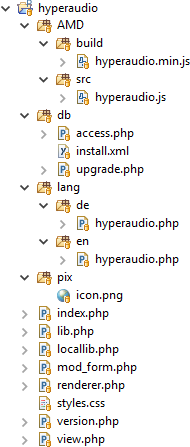
\includegraphics[width=0.3\textwidth,center]{Ordnerstruktur.PNG}
\caption{\label{fig:Ordnerstruktur}Ordnerstruktur des Hyperaudio-Plugins}
\end{figure}

\todo[inline]{Ordnerstruktur aktualisieren}

Im Ordner \textbf{/hyperaudio/backup} werden die Dateien abgelegt, welche Anwendung finden, wenn ein Backup oder eine Wiederherstellung eines Kurses vorgenommen wird.

Der Ordner \textbf{/hyperaudio/db} beherbergt die Dateien \textbf{access.php}, \textbf{events.php}, \textbf{install.xml} und \textbf{upgrade.php}. Die Datei \textbf{access.php} dient zur Steuerung der Berechtigungen innerhalb des Moodle-Plugins, wobei den verschiedenen Moodle-Rollen verschiedene Rechte für die einzelnen Funktionen zugewiesen werden können. In der \textbf{events.php} können Beobachter eingerichtet werden, welche auf bestimmte Ereignisse warten. Bei der Installation des Plugins wird die \textbf{install.xml} zur Erstellung der Datenbanktabellen für das Plugin verwendet. Es ist mindestens eine Tabelle mit dem Namen des Plugins anzulegen. Sollten die Datenbanktabellen nach Veröffentlichung des Plugins um Spalten erweitert werden, so kommt die Datei \textbf{upgrade.php} zum Einsatz. Hierin werden die notwendigen Schritte für einen Versionsabgleich definiert.

Im Ordner \textbf{/hyperaudio/lang} wird die Sprachlokalisierung vorgenommen. Für jede Sprache wird innerhalb des \textbf{lang}-Ordners ein eigener Unterordner angelegt. Darin befindet sich jeweils eine PHP-Datei, in welcher die Übersetzungen definiert werden. Der Name dieser Datei entspricht wiederum dem Namen des Plugins.

Das Icon, welches für das Plugin  verwendet werden soll, muss im Ordner \textbf{/hyperaudio/pix} mit dem Dateinamen \textbf{icon.gif} abgelegt werden und sollte eine Auflösung von 16x16 Pixel besitzen.

Im Ordner \textbf{/hyperaudio} liegen darüber hinaus die Dateien \textbf{lib.php}, \textbf{mod\underline{{ }}form.php}, \textbf{index.php}, \textbf{view.php} und \textbf{version.php}. Die \textbf{lib.php} dient dazu, Standardfunktionen von Moodle zu überschreiben, wobei \texttt{add\underline{{ }}instance}, \texttt{update\underline{{ }}instance} und \texttt{delete\underline{{ }}instance} als essenzielle Funktionen zu nennen sind. Mit diesen Funktionen wird das Anlegen, Aktualisieren und Löschen von Instanzen des Plugins ermöglicht. Zum Anlegen und Aktualisieren wird in der \textbf{mod\underline{{ }}form.php} die dazugehörige Maske festgelegt.Die \textbf{\textit{index.php}} dient der Auflistung aller Instanzen eines Plugins innerhalb eines Kurses. Je nach Umsetzung kann der Inhalt dieser Auflistung unterschiedlich viele Informationen zu den Instanzen bereitstellen. Auch ist es beispielsweise anhand von Berechtigungen aus der \textbf{access.php} möglich gewisse Inforationen nur bestimmten Usern anzuzeigen. Die erste Datei, die beim Öffnen der Aktivität geladen wird, ist die \textbf{view.php}, welche dementsprechend vornehmlich der Anzeige der Inhalte dient. In der \textbf{version.php} wird die Version des Plugins gepflegt. Erhöht sich die Versionsnummer in der \textbf{version.php}, wird der automatische Upgradeprozess von Moodle für das Plugin ausgelöst.

Neben diesen vorgegebenen Dateien kommen üblicherweise noch weitere Dateien bei der Entwicklung eines Moodle-Plugins zum Einsatz \citep{wild2017moodle}. Dazu gehört beispielsweise die \textbf{locallib.php}, in welcher üblicherweise alle plugineigenen PHP-Funktionen deklariert werden. Auch ist es Usus, die eigentliche Darstellung der Plugin-Inhalte innerhalb eines Kurses von der \textbf{view.php} in eine \textbf{renderer.php} zu verlagern. Dort können verschiedene Renderer-Klassen, welche durch Moodle bereitgestellt werden, für die eigenen Bedürfnisse überschrieben werden. Anpassungen optischer Natur können durch CSS (Cascading Style Sheets) in der \textbf{styles.css} vorgenommen werden. Eigene JavaScript-Module, welche beispielweise beim Laden der \textbf{view.php} automatisch aufgerufen werden, sind im Verzeichnis \textbf{/hyperaudio/AMD} (Asynchronous Module Definition) abzulegen.

%%%%%%%%%%
\section{Iterative Entwicklung}
Die Entwicklung des Plugins wird in iterativer Form durchgeführt. In jeder Iteration soll das Plugin nur um einige wenige Funktionalitäten erweitert werden. Jede Iteration soll mit einem lauffähigen Plugin abgeschlossen werden. So kann direkt das Ergebnis betrachtet werden und gegebenenfalls in der nächsten Iteration nochmals angepasst werden \citep{augsten2018iterativ}. Die Reihenfolge, in welcher die Funktionalitäten umgesetzt werden, leitet sich aus der Priorisierung der Anforderungen aus Abschnitt \ref{sec:anforderungsdefinition} ab.

\subsection{Speichern und Abspielen einer Audio-Datei}
\label{sec:it1}
In der ersten Iteration wird zunächst die grundlegende Struktur des Plugins erstellt (vgl. Abschnitt \ref{sec:architektur}). Ziel der ersten Iteration soll es sein, eine Audio-Datei speichern und wiedergeben zu können.

Dazu wird in der Maske zum Anlegen und Aktualisieren von Instanzen des Hyperaudio-Plugins (\textbf{mod\underline{{ }}form.php}) neben dem obligatorischen Namens-Feld noch ein Element zum Hinzufügen einer Audio-Datei angelegt. Auflistung \ref{lst:it1:modform} zeigt einen Ausschnitt des Codes, der in der Funktion \texttt{definition} der Klasse \texttt{mod\underline{{ }}hyperaudio\underline{{ }}mod\underline{{ }}form}, die von der Klasse \texttt{moodleform\underline{{ }}mod} erbt, ergänzt werden muss. 

\begin{lstlisting}[language=php,
             linewidth=\textwidth,
             caption={Ausschnitt der \textbf{mod\underline{{ }}form.php} in der 1. Iteration},
             label={lst:it1:modform}]
$mform = $this->_form;             
$mform->addElement('text', 'name', get_string('hyperaudio_mod_form_name',
    'hyperaudio'));
$mform->setType('name', PARAM_TEXT);
$mform->addRule('name', get_string('error_wrong_hyperaudio_name_input',
    'hyperaudio'), 'required');
$mform->addElement('filemanager', 'audiofile', get_string('hyperaudiodata',
    'hyperaudio'), null,
    array(
       'subdirs' => 0,
       'maxbytes' => 0,
       'areamaxbytes' => 10485760,
       'maxfiles' => 1,
       'accepted_types' => array('audio')
    )
);
$mform->addRule('audiofile', get_string('required', 'hyperaudio'), 'required');
\end{lstlisting}

Der \texttt{\underline{{ }}form} der \texttt{moodleform\underline{{ }}mod} können durch \texttt{addElement} neue Form-Elemente hinzugefügt werden. Mithilfe der Funktionen \texttt{setType} und \texttt{addRule} können den Elementen Datentypen und Regeln zugewiesen werden, die bei Auswertung der Form automatisch validiert werden. Zum Hochladen von Dateien kann der \textit{filemanager} eingesetzt werden. Mithilfe eines Arrays können dabei Einschränkungen für Anzahl und Eigenschaften der hochzuladenden Dateien festgelegt werden. In diesem Fall darf maximal eine Datei hinzugefügt werden, die vom Typ \textit{audio} sein muss. Die Funktion \texttt{get\underline{{ }}string} dient im Allgemeinen der Darstellung der lokalisierten Bezeichnungen.

Um die Daten aus der Form in der Datenbank speichern und später wieder löschen zu können, muss auch die \textbf{lib.php} bearbeitet werden. Dazu dienen die bereits erwähnten Funktionen \texttt{add\underline{{ }}instance}, \texttt{update\underline{{ }}instance} und \texttt{delete\underline{{ }}instance}. Beispielhaft wird in Auflistung \ref{lst:it1:lib} die Funktion \texttt{add\underline{{ }}instance} zum Hinzufügen eines neuen Hyperaudio-Dokuments betrachtet. 

\begin{lstlisting}[language=php,
             linewidth=\textwidth,
             caption={Ausschnitt der \textbf{lib.php} in der 1. Iteration},
             label={lst:it1:lib}]
function hyperaudio_add_instance($data) {
    global $DB;
    
    $cmid = $data->coursemodule;
    $context = context_module::instance($cmid);
    
    $draftitemid_audiofile = $data->audiofile;
    unset($data->audiofile);
     
    $now = time();
    $data->timecreated = $now;
    $data->timemodified = $now;
    
    $data->id = $DB->insert_record('hyperaudio', $data);
    
    hyperaudio_update_audiofile($data->id, $context, $draftitemid_audiofile);
     
    return $data->id;
}
\end{lstlisting}

Der Parameter \texttt{\$data} enthält bereits die in der Form eingegebenen Daten. Das Attribut \mbox{\texttt{audiofile}} enthält nicht die Audio-Datei selbst, sondern die ID der \textit{draft file area} und soll im ersten Schritt nicht in der Tabelle \textit{hyperaudio} abgespeichert werden (vgl. Zeilen 7-8). Vor dem Speichern wird noch der aktuelle Zeitstempel hinterlegt (vgl. Zeilen 10-12). Mithilfe der Funktion \mbox{\texttt{\$DB->insert_record}} kann das \texttt{\$data}-Objekt mit seinen Attributen in der Tabelle \textit{hyperaudio} abgelegt werden. Im Nachhinein sorgt die in der \textbf{locallib.php} definierte Funktion \mbox{\texttt{hyperaudio_update_audiofile}} dafür, dass die Audio-Datei in der \textit{files}-Tabelle abgespeichert und in der \textit{hyperaudio}-Tabelle korrekt referenziert wird (vgl. Auflistung \ref{lst:it1:locallib}).

\begin{lstlisting}[language=php,
             linewidth=\textwidth,
             caption={Ausschnitt der \textbf{locallib.php} in der 1. Iteration},
             label={lst:it1:locallib}]
function hyperaudio_update_audiofile($hyperaudioid, $context, $draftitemid) {
    global $DB;
    
    file_save_draft_area_files($draftitemid, $context->id, 'mod_hyperaudio',
    'audiofile', $hyperaudioid);
    $fs = get_file_storage();
    $files = $fs->get_area_files($context->id, 'mod_hyperaudio', 'audiofile',
    $hyperaudioid, 'itemid, filepath, filename', false);

    $file = reset($files);
    $DB->set_field('hyperaudio', 'audiofile', $file->get_filename(), array(
        'id' => $hyperaudioid
    ));
}
\end{lstlisting}

Wie bereits in Abschnitt \ref{sec:architektur} angedeutet, übernimmt die \textbf{renderer.php} die Anzeige der Hyperaudio-Inhalte (siehe Auflistung \ref{lst:it1:renderer}). Die \textbf{view.php} dagegen reduziert sich auf wenige Zeilen (vgl. Auflistung \ref{lst:it1:view}). Der Plugin-Renderer wird hier benutzt, um Header, Hauptinhalte und Footer anzuzeigen.

\begin{lstlisting}[language=php,
deletekeywords={header},
             linewidth=\textwidth,
             caption={Ausschnitt der \textbf{view.php} in der 1. Iteration},
             label={lst:it1:view}]
$output = $PAGE->get_renderer('mod_hyperaudio');
echo $output->header();
echo $output->display($hyperaudio, $context);
echo $output->footer();
\end{lstlisting}

In der Funktion \texttt{display} der Klasse \mbox{\texttt{mod_hyperaudio_renderer}}, die von der Klasse \mbox{\texttt{plugin_renderer_base}} erbt, werden die HTML-Inhalte erzeugt. Dabei handelt es sich in der 1. Iteration um einen Container, der ein \texttt{<audio>}-Element beinhaltet. Als Quelle wird im \texttt{<source>}-Element eine URL (Uniform Resource Locator) angegeben, die zuvor mit Moodle-Standardmitteln erzeugt wurde und auf die in der Datenbank abgelegte Audio-Datei verweist.

\begin{lstlisting}[language=php,
             linewidth=\textwidth,
             caption={Ausschnitt der \textbf{renderer.php} in der 1. Iteration},
             label={lst:it1:renderer}]
$audio_fileinfo = array(
    'component' => 'mod_hyperaudio',
    'filearea' => 'audiofile',
    'itemid' => $hyperaudio->id,
    'contextid' => $context->id,
    'filepath' => '/',
    'filename' => $hyperaudio->audiofile
);

$audiofileurl = moodle_url::make_pluginfile_url(
    $audio_fileinfo['contextid'], $audio_fileinfo['component'],
    $audio_fileinfo['filearea'], $audio_fileinfo['itemid'],
    $audio_fileinfo['filepath'], $audio_fileinfo['filename']);
$audio_url = $audiofileurl->get_scheme() . '://' . $audiofileurl->get_host() . $audiofileurl->get_path();
if ($audiofileurl->get_port()){
    $audio_url .= ':' . $audiofileurl->get_port();
}

$output = '<div id="hyperaudio" data-hyperaudio_id="'.$hyperaudio->id.'">';
$output .= '<audio id="hyperaudio_audio" controls style="width:800px;">' .
    '<source src="' . $audio_url . '"/>' .
    '</audio>';
$output .= '</div>';

echo $output;
\end{lstlisting}

Auf die beschriebene Art und Weise lässt sich ein Hyperaudio-Dokument, das vorläufig allein aus einer Audio-Datei besteht, speichern und mithilfe des HTML5-Audio-Players wiedergeben.


\subsection{Speichern und Anzeige von Zusatzinhalten}
Bei der zweiten Iteration wird das Plugin um die Möglichkeit zum Speichern und zeitabhängigen Anzeigen der Zusatzinhalte erweitert. Für das Speichern wird analog zu Abschnitt \ref{sec:it1} vorgegangen. Es wird ein Filemanager (\textbf{mod\underline{{ }}form}) ergänzt, welcher das Hochladen von beliebig vielen Bilddateien erlaubt. Zusätzlich wird die \textbf{locallib.php} um die Funktionen \mbox{\texttt{hyperaudio_update_additional_content}} und \mbox{\texttt{hyperaudio_delete_additional_content}} erweitert. Die Löschfunktion dient dazu zu verhindern, dass beispielsweise beim Ergänzen von Zusatzinhalten, die bereits vorhanden Zusatzinhalte erneut abgespeichert werden. Dementsprechend wird diese Funktion, wie in Auflistung \ref{lst:it2:locallib} zu sehen, innerhalb der Funktion \mbox{\texttt{hyperaudio_update_additional_content}} aufgerufen. Die Zeilen 19 bis 24 dienen dazu die Metadaten des Zusatzinhaltes festzuhalten, in dieser Iteration werden diese noch manuelle mit Beispieldaten befüllt. Die Funktion \mbox{\texttt{hyperaudio_update_additional_content}} wird dann entsprechend bei den Funktionen \texttt{add\underline{{ }}instance} und \texttt{update\underline{{ }}instance} innerhalb der \textbf{lib.php} ergänzt.

\begin{lstlisting}[language=php,
             linewidth=\textwidth,
             caption={Ausschnitt der \textbf{locallib.php} in der 2. Iteration},
             label={lst:it2:locallib}]
function hyperaudio_update_additional_content($hyperaudioid, $context, $draftitemid, $configfile) {
	global $DB;
    
	hyperaudio_delete_additional_content($hyperaudioid, $context);
    
	file_save_draft_area_files($draftitemid, $context->id, 'mod_hyperaudio', 'additional_content', $hyperaudioid);
	$fs = get_file_storage();
    
	$files = $fs->get_area_files($context->id, 'mod_hyperaudio', 'additional_content', $hyperaudioid, 'itemid, filepath, filename',
            false);
	$counter=1;
	$begin=0;
	$end=10;
	foreach ($files as $file) {        
		$additional_content = new \stdClass();
		$additional_content->file = $file->get_filename();
		$additional_content->hyperaudio_id = $hyperaudioid;
        
		$additional_content->name = 'Name: '.$counter;
		$additional_content->course_unit = 'Kurseinheit: '.$counter;
		$additional_content->page = 'Seite: '.$counter;
		$additional_content->description = 'Beschreibung: '$counter;
		$additional_content->begin = $begin;
		$additional_content->end = $end;
        
		$now = time();
		$additional_content->timecreated = $now;
		$additional_content->timemodified = $now;
        
		$additional_content_id = $DB->insert_record('additional_content', $additional_content);
		
		$counter++;
		$begin+=15;
		$end+=15;
    }
}
\end{lstlisting}

Nachdem nun die Zusatzinhalte samt der Metadaten gespeichert sind, kann sich der zeitabhänigen Darstellung dieser beim Abspielen der Audio-Datei zugewendet werden. An dieser Stelle findet nun das JavaScript-Framework \textit{Popcorn.js} seine Anwendung, da dies wie bereits in Abschnitt \ref{sec:Technik} beschrieben, das zeitabhängige Annotieren von Inhalten ermöglicht. Um \textit{Popcorn.js} und dessen \textit{Images}-Plugin nutzen zu können, werden beide JavaScript Dateien in dem Ordner \textbf{/hyperaudio/thirdparty} abgelegt. Anschließend werden diese in die \textbf{view.php} eingebunden (siehe Auflistung \ref{lst:it2:view}).

\begin{lstlisting}[language=php,
             linewidth=\textwidth,
             caption={Ausschnitt der \textbf{view.php} in der 2. Iteration},
             label={lst:it2:view}]
$PAGE->requires->js('/mod/hyperaudio/thirdparty/popcorn.js', true);
$PAGE->requires->js('/mod/hyperaudio/thirdparty/popcorn.image.js', true);
\end{lstlisting}

Der eigentliche Einsatz von \textit{Popcorn.js} findet im Renderer statt. Hierfür wird der Code aus der ersten Iteration um ein neues \texttt{div} erweitert, in welchem die Zusatzinhalte angezeigt werden sollen. Darauf werden zunächst alle zugehörigen Zusatzinhalte geladen und ein Link zu diesem generiert (Zielen 9 bis 32 in Abbildung \ref{lst:it2:renderer}). Beim Aufruf des \textit{Popcorn.js} \textit{Images}-Plugins werden in Zeile 35 die Metadaten über Beginn und Ende der Anzeige sowie der generierte Link verwendet, um den Zusatzinhalt zum gewünschten Zeitpunkt im dafür erstellten \texttt{div} darzustellen.

\begin{lstlisting}[language=php,
             linewidth=\textwidth,
             caption={Ausschnitt der \textbf{renderer.php} in der 2. Iteration},
             label={lst:it2:renderer}]
$output = '<div id="hyperaudio" data-hyperaudio_id="'.$hyperaudio->id.'">';
$output .= '<div id="hyperaudio_additional_content" style="height:600px; width:800px;"></div>';
$output .= '<audio id="hyperaudio_audio" controls style="width:800px;">' . '<source src="' . $audio_url . '"/>' . '</audio>';

$output .= '<script type="text/javascript">' . 'document.addEventListener("DOMContentLoaded", function() {' .
		'var popcorn = Popcorn("#hyperaudio_audio");';

$files = hyperaudio_get_additional_content($hyperaudio->id, $context);
foreach ($files as $file) {
	$additional_content = $DB->get_record('additional_content', array(
		'hyperaudio_id' => $hyperaudio->id,
		'file' => $file->get_filename()
	), '*', IGNORE_MISSING);
	
	if ($additional_content == false){
		continue;
	}
	
	$additional_content_fileinfo = array(
		'component' => 'mod_hyperaudio',
		'filearea' => 'additional_content',
		'itemid' => $hyperaudio->id,
		'contextid' => $context->id,
		'filepath' => '/',
		'filename' => $additional_content->file
	);
	
	$additional_content_fileurl = moodle_url::make_pluginfile_url($additional_content_fileinfo['contextid'], $additional_content_fileinfo['component'], $additional_content_fileinfo['filearea'],
		$additional_content_fileinfo['itemid'], $additional_content_fileinfo['filepath'], $additional_content_fileinfo['filename']);
	$additional_content_url = $additional_content_fileurl->get_scheme() . '://' . $additional_content_fileurl->get_host() . $additional_content_fileurl->get_path();
	if ($additional_content_fileurl->get_port()){
		$additional_content_url .= ':' . $additional_content_fileurl->get_port();
	}
	
	$output .= 'popcorn.image({start: '.$additional_content->begin.', end: '.$additional_content->end.', href: "javascript:void(0);", src: "'.$additional_content_url.'", target: "hyperaudio_additional_content"});';
}

$output .= '}, false);</script>';
$output .= '</div>';

echo $output;
\end{lstlisting}

Mit diesen Erweiterungen wurde das Ziel dieser Iteration erreicht. Es ist nun möglich Zusatzinhalte abzuspeichern und diese unter Verwendung von \textit{Popcorn.js} zeitabhängig zur Audi-Datei darstellen zu lassen

\subsection{Einbindung der Konfigurationsdatei}
Während zum aktuellen Stand die Metadaten der Zusatzinhalte noch manuell im Code gepflegt werden, sollen dies mittels dieser Iteration aus einer Konfigurationsdatei ausgelesen werden. Am Anfang dieser Iteration steht erneut die Erweiterung der \textbf{mod\underline{{ }}form} um einen weiteren Filemanger. Die Speicherung verläuft analog zu der der Zusatzinhalte, mit der Einschränkung, dass nur eine Konfigurationsdatei im JSON-Format gespeichert werden kann. In diesem Zuge wird also erneut die \textbf{lib.php} entsprechend erweitert. Innerhalb der \textbf{lib.php} werden die Funktionen \texttt{hyperaudio\underline{{ }}update\underline{{ }}hyperaudio\underline{{ }}config} und \texttt{hyperaudio\underline{{ }}delete\underline{{ }}hyperaudio\underline{{ }}config} ergänzt. Des Weiteren wird, wie in Auflistung \ref{lst:it3:locallib} zu erkennen, die Funktion \texttt{hyperaudio\underline{{ }}update\underline{{ }}additional\underline{{ }}content} erweitert. Es ist ersichtlich, dass zunächst in Zeile 4 die Inhalte der Konfigurationsdatei ausgelesen werden, um diese Metadaten dann beim Abspeichern der Zusatzinhalte zu verwenden.

\todo[inline]{warum ist hier die delete Funktion notwendig?}

\begin{lstlisting}[language=php,
             linewidth=\textwidth,
             caption={Ausschnitt der \textbf{locallib.php} in der 3. Iteration},
             label={lst:it3:locallib}]
function hyperaudio_update_additional_content($hyperaudioid, $context, $draftitemid, $configfile) {
    global $DB;
    
    $additional_contents_data = parse_hyperaudio_config($hyperaudioid, $context, $configfile);
    
    hyperaudio_delete_additional_content($hyperaudioid, $context);
    
    file_save_draft_area_files($draftitemid, $context->id, 'mod_hyperaudio', 'additional_content', $hyperaudioid);
    $fs = get_file_storage();
    
    $files = $fs->get_area_files($context->id, 'mod_hyperaudio', 'additional_content', $hyperaudioid, 'itemid, filepath, filename',
            false);
    foreach ($files as $file) {        
        $additional_content = new \stdClass();
        $additional_content->file = $file->get_filename();
        $additional_content->hyperaudio_id = $hyperaudioid;
        
        $additional_content_data = $additional_contents_data[$additional_content->file];
        
        $additional_content->name = $additional_content_data->name;
        $additional_content->course_unit = $additional_content_data->course_unit;
        $additional_content->page = $additional_content_data->page;
        $additional_content->description = $additional_content_data->description;
        $additional_content->begin = $additional_content_data->begin;
        $additional_content->end = $additional_content_data->end;
        
        $now = time();
        $additional_content->timecreated = $now;
        $additional_content->timemodified = $now;
        
        $additional_content_id = $DB->insert_record('additional_content', $additional_content);
    }
}
\end{lstlisting}

Nachdem nun also die Zusatzinhalte mit den korrekten Metadaten versorgt sind, können diese im Renderer für die gesteuerte Darstellung mittels \textit{Popcorn.js} verwendet werden. Somit werden dank dieser Iteration die Zusatzinhalte nun zu den Zeitpunkten dargestellt, welche in der Konfigurationsdatei festgelegt sind.

\subsection{Speichern und Anzeige von Kommentaren}
Nachdem in den vorherigen Iterationen die Pflege und das Abspielen von Hyperaduio-Dokumenten im Fokus lag, konzentriert sich diese Iteration auf die Kommentarfunktion. Zu diesem Zweck wird im ersten Schritt der Renderer um entsprechende Elemente ergänzt, welche in Auflistung \ref{lst:it4:renderer} zu sehen sind. Bei den Elementen handelt es sich zum einen um ein Input-Feld mit dazugehörigen Submit-Button. Diese Elemente dienen dem Erstellen von Kommentaren. Das Element \texttt{<div id="hyperaudio_comments"></div>} soll der Anzeige der Kommentare dienen.
\todo[inline]{Problem mit "> lösen}

\begin{lstlisting}[language=php,
             linewidth=\textwidth,
             caption={Ausschnitt der \textbf{renderer.php} in der 4. Iteration},
             label={lst:it4:renderer}]
$output .=
	'<div>
		<label>'.get_string('mod_hyperaudio_renderer_comment', 'hyperaudio').':
			<input type="text" id="hyperaudio_comment" name="comment" autocomplete="off"/>
			<button type="button" class="comment_submit" data-comment_type="'.CommentType::Comment.'">'.get_string('mod_hyperaudio_renderer_submit_comment', 'hyperaudio').'</button>
		</label>
	</div>';
$output .= '<div id="hyperaudio_comments"></div>';
\end{lstlisting}

Das Speichern als auch das Anzeigen der Kommentare wird unter dem Einsatzes von Webservices, welche durch ein JavaScrip-Modul (\textbf{/hyperaudio/AMD/src/comnments.js}) angesprochen werden, umgesetzt. Hierfür werden zusätzlich die \textbf{services.php} (\textbf{/hyperaudio/db}) und \textbf{external.php} (\textbf{/hyperaudio/classes}) für die Bereitstellung der Webservices benötigt.

In der \textbf{services.php} werden zunächst die benötigten Webservices beschrieben (siehe Auflistung \ref{lst:it5:services}). Wie zu erkennen ist, wird hier lediglich auf die \textbf{external.php} verwiesen, in welcher der eigentliche Code des Webservices erstellt werden muss.

\begin{lstlisting}[language=php,
             linewidth=\textwidth,
             caption={\textbf{services.php} in der 5. Iteration},
             label={lst:it5:services}]
$functions = array(
	'mod_hyperaudio_save_comment' => array(
		'classname'   => 'mod_hyperaudio_external',
		'methodname'  => 'save_comment',
		'classpath'   => 'mod/hyperaudio/classes/external.php',
		'description' => 'Save comment',
		'type'        => 'write'
	),
	'mod_hyperaudio_load_comments' => array(
		'classname'   => 'mod_hyperaudio_external',
		'methodname'  => 'load_comments',
		'classpath'   => 'mod/hyperaudio/classes/external.php',
		'description' => 'Load comments',
		'type'        => 'read'
	)
);
\end{lstlisting}

In der \textbf{external.php} werden in der \texttt{mod_hyperaudio_external extends}, welche von der Klasse \texttt{external_api} erbt (vgl. Auflistung \ref{lst:it5:external}), die nötigen Funktionen definiert. Beim Speichern von Kommentaren sind dies die Funktionen \texttt{save_comment_parameters}, \texttt{save_comment_is_allowed_from_ajax}, \texttt{save_comment} und \texttt{save_comment_returns}. In der ersten Funktion werden die Parameter, welche benötigt werden definiert. In der zweiten Funktion wird festgelegt, ob die Funktion durch \textit{AJAX} ( Asynchronous JavaScript and XML) aufgerufen werden darf, dies ist für das geplante Vorgehen innerhalb des Hyperaudio-Plugins nötigt. In der Funktion \texttt{save_comment} wird die eigentliche Funktionalität des Webservices programmiert. In diesem Fall also das Speichern des Kommentars in der Datenbank. In der vierten Funktion werden die Rückgabeparamter des Webservices beschrieben. Im Fall der Funktion \texttt{load_comments_returns} also die Kommentare, welche angezeigt werden sollen.

\begin{lstlisting}[language=php,
             linewidth=\textwidth,
             caption={\textbf{external.php} in der 5. Iteration},
             label={lst:it5:external}]
class mod_hyperaudio_external extends external_api {
    
	public static function load_comments_parameters() {
		return new external_function_parameters(
			array(
				'hyperaudio_id' => new external_value(PARAM_INT, 'hyperaudio_id')
			)
		);
	}
    
	public static function load_comments_is_allowed_from_ajax() {
		return true;
	}
    
	public static function load_comments($hyperaudio_id) {
		global $CFG, $DB, $USER;
        
		require_once ($CFG->dirroot . '/mod/hyperaudio/locallib.php');
		require_once ($CFG->dirroot . '/mod/hyperaudio/classes/enums.php');
        
		$comments = $DB->get_records_sql(
			'SELECT comments.id, comments.comment_type, comments.commenttext, comments.timeannotated, comments.timecreated, user.username, comments.comment_id'.
			' FROM mdl_hyperaudio_comments comments'.
			' INNER JOIN mdl_user user ON comments.userid = user.id'.
			' LEFT JOIN mdl_hyperaudio_comments original_comment ON original_comment.id = comments.comment_id'.
			' WHERE comments.hyperaudio_id = ?'.
			' AND (comments.comment_type = ? OR (comments.comment_type =? AND comments.userid = ?))'.
			' ORDER BY IFNULL(original_comment.timecreated, comments.timecreated)*POWER(10, 11) + comments.timecreated',
			array($hyperaudio_id, CommentType::Comment, CommentType::Note, $USER->id)
			);
        
		$result_comments = array();
		foreach ($comments as $comment) {
			$result_comment = array(
				'id' => $comment->id,
				'username' => $comment->username,
				'date' => date('d.m.Y H:i', $comment->timecreated),
				'time' => format_time_annotated($comment->timeannotated),
				'text' => $comment->commenttext,
				'comment_type_display' => CommentType::get_comment_type($comment->comment_type),
				'comment_type' => $comment->comment_type,
				'comment_id' => $comment->comment_id
			);
			$result_comments[] = $result_comment;
		}
        
		return $result_comments;
    }
    
	public static function load_comments_returns() {
		return new external_multiple_structure(
			new external_single_structure(
				array(
					'id' => new external_value(PARAM_INT, 'id'),
					'username' => new external_value(PARAM_TEXT, 'username'),
					'date' => new external_value(PARAM_TEXT, 'date'),
					'time' => new external_value(PARAM_TEXT, 'time'),
					'text' => new external_value(PARAM_TEXT, 'text'),
					'comment_type_display' => new external_value(PARAM_TEXT, 'comment_type_display'),
					'comment_type' => new external_value(PARAM_TEXT, 'comment_type'),
					'comment_id' => new external_value(PARAM_INT, 'comment_id')
				)
			)
		);
	}

	public static function save_comment_parameters() {
		return new external_function_parameters(
			array(
				'comment' => new external_value(PARAM_TEXT, 'comment'),
				'hyperaudio_id' => new external_value(PARAM_INT, 'hyperaudio_id'),    
				'timeannotated' => new external_value(PARAM_INT, 'timeannotated'),
				'comment_type' => new external_value(PARAM_TEXT, 'comment_type')                                               
			)
		);
	}

	public static function save_comment_is_allowed_from_ajax() {
		return true;
	}

	public static function save_comment($comment, $hyperaudio_id, $timeannotated, $comment_type) {
		global $CFG, $DB, $USER;
        
		require_once ($CFG->dirroot . '/mod/hyperaudio/classes/enums.php');
                    
		$hyperaudio_comment = new \stdClass();
		$hyperaudio_comment->hyperaudio_id = $hyperaudio_id;
		$hyperaudio_comment->userid = $USER->id;
		$hyperaudio_comment->timeannotated = $timeannotated;
		$hyperaudio_comment->comment_type = $comment_type;
        
		if ($comment_type == CommentType::Comment || $comment_type == CommentType::Note){
			$hyperaudio_comment->commenttext = $comment;
		}
        
		$now = time();
		$hyperaudio_comment->timecreated = $now;
		$hyperaudio_comment->timemodified = $now;
        
		$DB->insert_record('hyperaudio_comments', $hyperaudio_comment);
        
		return 0;
    }
    
	public static function save_comment_returns() {
		return new external_value(PARAM_INT, '0 = ok, 1 = error');
	}
}             
\end{lstlisting}
\todo[inline]{Listing anpassen, speziell SQL-Statement auf die nur Kommentare-Variante kürzen}

Auf die mittels \textbf{services.php} und \textbf{external.php} bereitgestellten Webservice wird letztlich in der \textbf{comments.js} zugegriffen, um die im Renderer definierten Elemente zu befüllen, beziehungsweise deren Inhalte auszulesen. Die Funktion zum Speichern eines Kommentars ist exemplarisch in Auflistung \ref{lst:it5:comments} dargestellt. Zunächst werden die im Renderer erstellten Elemente zum Erstellen eines Kommentars ausgelesen, dann wird mittels eines AJAX-Calls der Webservice \texttt{mod_hyperaudio_save_comment} aufgerufen und die benötigten Parameter übergeben. Hierbei ist hervorzuheben, dass der Zeitpunkt zu dem der Kommentar an das Hyperaudio-Dokument annotiert wird über die Funktion \texttt{currentTime} des \textit{Popcorn.js}-Frameworks ermittelt wird. Bei der Funktion zum Darstellen der Kommentare wird analog vorgegangen, nur dass mittels des Webservices die Kommentare für das betroffene Hyperaudio-Dokumente aufgerufen werden und dann innerhalb des entsprechenden Elements des Renderers dargestellt werden.

\begin{lstlisting}[language=php,
             linewidth=\textwidth,
             caption={Ausschnitt der \textbf{comments.js} in der 5. Iteration},
             label={lst:it5:comments}]
function save_comment(comment_type){
	var comment = $("#hyperaudio_comment").val();
	var hyperaudio_id = get_hyperaudio_id();
	var popcorn = Popcorn("#hyperaudio_audio");
	var timeannotated = popcorn.currentTime();
	timeannotated = parseInt(timeannotated);
	    
	var promises = ajax.call([{
		methodname: 'mod_hyperaudio_save_comment',
		args:{
			'comment': comment,
			'hyperaudio_id': hyperaudio_id,       
			'timeannotated': timeannotated,
			'comment_type': comment_type
		}
	}]);
	promises[0].done(function(data) {
		show_comments();
	});
}
\end{lstlisting}
\todo[inline]{Sprache des Listings anpassen}

Mit dem Abschluss dieser Iteration wurde die Möglichkeit geschaffen Kommentar zu erstellen und den Zeitpunkt innerhalb des Hyperaduio-Dokuments festzuhalten, zu dem der Kommentar erstellt wurde. Im gleichen Zuge wurde auch die Darstellung dieser Kommentare ermöglicht.

\subsection{Antworten auf Kommentare}
Während bereits Kommentare verfasst und angezeigt werden können, fehlt noch die Möglichkeit auf diese zu antworten. Diese Funktionalität wird in dieser Iteration ergänzt. Zu diesem Zweck wird ein neuer Webservices zum Speichern von Antworten erstellt und der Webservice zum Darstellen der Kommentare um die Antworten erweitert. Demzufolge wird in der \textbf{services.php} eine Beschreibung für den neuen Webservice zum Erstellen von Antworten ergänzt und in der \textbf{external.php} werden die vier Funktionen analog zum Webservice zum Speichern Kommentaren ergänzt. Bei der \textbf{comments.js} bedarf es ebenfalls nur kleinere Anpassungen, unter anderem um die Anzeige eines Antworten Buttons und eines Textfeldes bei dessen Betätigung zu ermöglichen. Die hierfür notwendige Erweiterung innerhalb der Funktion \texttt{show_comments} ist in der Auflistung \ref{lst:it6:comments} zu sehen.

\begin{lstlisting}[language=php,
             linewidth=\textwidth,
             caption={Ausschnitt der \textbf{comments.js} in der 6. Iteration},
             label={lst:it6:comments}]
if (this.comment_type === CommentType.Comment && !this.comment_id){
	output = output + '<div class="comment_answer comment_actions" data-comment_id="'+this.id+'">';
	output = output + '<a href="javascript:void(0);" class="comment_answer_link comment_link" onclick="show_answer_input(this)" data-comment_id="'+this.id+'">' + string_answer + '</a>';
	output = output + '<input type="text" class="comment_answer_text comment_hidden_element" data-comment_id="'+this.id+'"/>';
	output = output + '<button type="button" class="comment_answer_button comment_hidden_element" data-comment_id="'+this.id+'">' + string_answer + '</button>';
	output = output + '</div>';
\end{lstlisting}

Die Darstellung der Antworten und deren Zuordnung zu den dazugehörigen Kommentaren wird durch die in Auflistung \ref{lst:it6:external} ersichtlichen Anpassung des SQL-Statements \texttt{load_comments}-Funktion innerhalb der \textbf{external.php} erreicht.

\begin{lstlisting}[language=php,
             linewidth=\textwidth,
             caption={Ausschnitt der \textbf{external.php} in der 6. Iteration},
             label={lst:it6:external}]
$comments = $DB->get_records_sql(
	'SELECT comments.id, comments.comment_type, comments.commenttext, comments.timeannotated, comments.timecreated, user.username, comments.comment_id'.
	' FROM mdl_hyperaudio_comments comments'.
	' INNER JOIN mdl_user user ON comments.userid = user.id'.
	' LEFT JOIN mdl_hyperaudio_comments original_comment ON original_comment.id = comments.comment_id'.
	' WHERE comments.hyperaudio_id = ?'.
	' AND (comments.comment_type = ? OR (comments.comment_type =? AND comments.userid = ?))'.
	' ORDER BY IFNULL(original_comment.timecreated, comments.timecreated)*POWER(10, 11) + comments.timecreated',
	array($hyperaudio_id, CommentType::Comment, CommentType::Note, $USER->id)
);
\end{lstlisting}

Durch die Erweiterungen und Anpassungen innerhalb dieser Iteration ist es nun möglich auf Kommentare zu antworten und diese Antwort bei dem zugehörigen Kommentar darzustellen.

\todo[inline]{SQL-Statement auf Kommentare und Antworten kürzen}
\todo[inline]{Abkürzung SQL muss schon früher kommen}

\subsection{Notizen}
Nachdem durch die vorangegangen Iterationen nun die Funktionen für die Kommunikation zwischen Studierenden und Lehrenden geschaffen wurden, zielt diese Iteration auf das Erstellen und Darstellen von Notizen ab.

Im ersten Schritt wird hierfür in der \textbf{renderer.php} die Erweiterung um einen weiteren dedizierten Button entsprechend der Auflistung \ref{lst:it7:renderer} vorgenommen.

\begin{lstlisting}[language=php,
             linewidth=\textwidth,
             caption={Ausschnitt der \textbf{renderer.php} in der 7. Iteration},
             label={lst:it7:renderer}]
$output .=
	'<div>
		<label>'.get_string('mod_hyperaudio_renderer_comment', 'hyperaudio').':
			<input type="text" id="hyperaudio_comment" name="comment" autocomplete="off"/>
			<button type="button" class="comment_submit" data-comment_type="'.CommentType::Comment.'">'.get_string('mod_hyperaudio_renderer_submit_comment', 'hyperaudio').'</button>
			<button type="button" class="comment_submit" data-comment_type="'.CommentType::Note.'">'.get_string('mod_hyperaudio_renderer_submit_note', 'hyperaudio').'</button>
		 </label>
	</div>';
\end{lstlisting}

Nachdem diese Anpassung vorgenommen wurde, können zum Speichern der Notizen die gleichen Webservices und Funktionen, wie zum Speichern der Kommentare verwendet werden. Dies rührt daher, dass Notizen als eine bestimmte Art von Kommentaren angesehen wird (vgl. Abschnitt \ref{sec:komponenten_zusammenhaenge}). Zum Darstellen der Notizen wird, wie bereits in der vorherigen Iteration für die Antworten, das SQL-Statement in der \texttt{load_comments} der \textbf{external.php} angepasst.

Da Notizen im Gegensatz zu Kommentaren geändert und gelöscht werden können sollen, müssen hierfür entsprechende Webservices bereitgestellt werden (siehe Auflistung \ref{lst:it7:services}).

\begin{lstlisting}[language=php,
             linewidth=\textwidth,
             caption={Ausschnitt der \textbf{services.php} in der 7. Iteration},
             label={lst:it7:services}]
'mod_hyperaudio_save_note_edit' => array(
        'classname'   => 'mod_hyperaudio_external',
        'methodname'  => 'save_note_edit',
        'classpath'   => 'mod/hyperaudio/classes/external.php',
        'description' => 'Save note edit',
        'type'        => 'write'
    ),
    'mod_hyperaudio_delete_comment' => array(
        'classname'   => 'mod_hyperaudio_external',
        'methodname'  => 'delete_comment',
        'classpath'   => 'mod/hyperaudio/classes/external.php',
        'description' => 'Delete comment',
        'type'        => 'write'
    )
\end{lstlisting}

 Wie bereits am Namen des Webservices erkennbar, wird dieser theoretisch in der Lage sein, alle Arten von Kommentaren löschen zu können. Der dazugehörig Button wird jedoch nur bei Notizen dargestellt. Dies wird mittels der Bedingung aus Auflistung \ref{lst:it7:comments} innerhalb der \textbf{comments.js} erreicht.
 
\begin{lstlisting}[language=php,
             linewidth=\textwidth,
             caption={Ausschnitt der \textbf{comments.js} in der 7. Iteration},
             label={lst:it7:comments}]
else if (this.comment_type === CommentType.Note){
	output = output + '<div class="comment_note comment_actions" data-comment_id="'+this.id+'">';
	output = output + '<a href="javascript:void(0);" class="comment_note_edit_link comment_link" onclick="show_note_edit_input(this)" data-comment_id="'+this.id+'">' + string_edit + '</a>';
	output = output + '<a href="javascript:void(0);" class="comment_note_delete_link comment_link" data-comment_id="'+this.id+'">' + string_delete + '</a>';
	output = output + '<input type="text" class="comment_note_edit_text comment_hidden_element" data-comment_id="'+this.id+'"/>';
	output = output + '<button type="button" class="comment_note_edit_button comment_hidden_element" data-comment_id="'+this.id+'">' + string_edit + '</button>';
	output = output + '</div>';
}
\end{lstlisting}

Entsprechend der Webservices werden innerhalb der \textbf{external.php} Funktionen zum Editieren von Notizen und dem Löschen von Kommentaren erstellt. Damit sind alle nötigen Schritte durchgeführt um Notizen erstellen, anzeigen und löschen zu können.

\subsection{Audio Cues}
Das Abspielen der Audio Cues im Moment der Darstellung eines Zusatzinhaltes wird durch eine Anpassung an dem verwendeten \textit{Popcorn.js}-Plugins \textit{Images} erreicht. Zu diesem Zweck wird der Code aus Zeile 6 bis 7  aus Auflistung \ref{lst:it8:popcorn.image} ergänzt. Mit diesen Zeilen wird ein Audio Element erstellt und abgespielt. Diese Anpassung wird innerhalb der Funktion \texttt{start} vorgenommen, also in der Funktion, die ausgeführt wird, wenn die Darstellung des Zusatzinhalts beginnen soll.

\begin{lstlisting}[language=php,
             linewidth=\textwidth,
             caption={Ausschnitt der \textbf{popcorn.image.js} in der 8. Iteration},
             label={lst:it8:popcorn.image}]
start: function( event, options ) {
	options.anchor.style.display = "inline";
	if ( options.trackedContainer ) {
		options.trackedContainer.start();
	}
	var audioElement = document.createElement('audio');
	audioElement.setAttribute('src', '../hyperaudio/ding.mp3');
	audioElement.play();
}
\end{lstlisting}

\subsection{Galerie der Zusatzinhalte}
\dots

\subsection{Zeitabhängige Visualisierung der Kommentare}
\dots

\subsection{Markierungen}
\dots

%\subsection{Suche, Filter und Sortierung bei Kommentaren}
%\dots
%
%\subsection{Export-/Import-Funktion}
%\dots

%TODO: Wiedergabe von Videos

%%%%%%%%%%
\section{Zusammenfassung}
\dots